\documentclass[11pt,a4paper,twocolumn]{article}
\usepackage[utf8]{inputenc}
\usepackage[T1]{fontenc}
\usepackage{amsmath}
\usepackage{amssymb}
\usepackage{amsfonts}
\usepackage{graphicx}
\usepackage[spanish]{babel}
\usepackage{booktabs,fourier,tabularx,wrapfig,multicol,multirow,caption, subcaption,tikz, fancyhdr,steinmetz,xcolor}
\usepackage[many]{tcolorbox}

\usepackage[left=2cm,right=2cm,top=2cm,bottom=2cm]{geometry}

\graphicspath{{../imageneselectro/}}

%Configuración y comandos

%BEGIN_FOLD
%tcolorbox personalizado
\newtcolorbox{cajita}{colback=white!97!brown, colframe=brown!15!gray, breakable}
%Prueba 
%BEGIN_FOLD
%\newtcolorbox{mybox}[1]{title = \textsc{Unidad #1},colbacktitle=red!85!black,enhanced,attach boxed title to top center={yshift=-2mm}, colbacktitle=white, coltitle=gray!50!black, boxed title style={colframe=blue!30},colback=white!97!brown, colframe=blue!30 }
%END_FOLD

%Encabezado y pie de página
\fancyhead[R]{\textsc{Electrotecnia}}
\fancyhead[L]{
\includegraphics[width=.1\textwidth]{utncom}}
\fancyhead[C]{Hoja de fórmulas}
\fancyfoot[R]{ \vspace{.1cm}| Página \thepage }
\fancyfoot[L]{\hrule \vspace{.1cm} Franzoi Valentin, Guardiani Franco, Polo Daiana}
\fancyfoot[C]{ \vspace{.1cm}}

%Comando para fasores :)
\newcommand{\fasor}[1]{\textit{\textbf{#1}}}

%Comando título de cada unidad
\newcommand{\unidad}[2]{\begin{center}
		\fontsize{10}{10}\selectfont\color{gray!50!black}\scshape Unidad #1 \\
		\fontsize{14}{14}\selectfont \scshape #2
\end{center} \vspace{-.6cm}}

%END_FOLD

\begin{document}
%	unidades 1 a 5
	%BEGIN_FOLD
\pagestyle{fancy}

	\section*{Nomenclatura}
	\begin{tabular}{r l}
		$R$ [$\Omega$] & Resistencia \\
		$C$ [F] & Capacitancia \\
		$L$ [H] & Inductancia \\
		$i$ [A] & Corriente \\
		$v$ [V] & Tensión o voltaje \\
		$w$ [J] & Energía almacenada \\
		$j$ & Unidad imaginaria \\
		$t$ [s] & Tiempo \\
		$LTK$ & Ley de Kirchhoff para la tensión \\
		$LCK$ & Ley de Kirchhoff para la corriente \\
		$P$[W] & Potencia \\
		$\fasor{Z}$ [$\Omega$]& Impedancia \\
		$X_{C}$ [$\Omega$] & Reactancia capacitiva \\
		$X_{L}$ [$\Omega$] & Reactancia inductiva \\
		$\tau$ [s] & Constante de tiempo \\
		$\alpha$ [$^\circ$/s]& Factor de amortiguamiento \\
		$\omega_{0}$ [$^\circ$/s] & Frecuencia natural no amortiguada \\
		$\omega_{d}$ [$^\circ$/s] & Frecuencia natural amortiguada \\
	\end{tabular}


	\unidad{1}{Teoría Elemental de los Circuitos}
	
	\begin{tcolorbox}[colback=white!97!brown, colframe=brown!15!gray]
		
		\begin{tabular}{r l}
			\textbf{Ley de Ohm} & $I=\dfrac{V}{R}$ \\
\vspace{.1cm}	Corriente en el capacitor & $i_{C}=C \dfrac{dv}{dt}$ \\
\vspace{.1cm}	Voltaje en el inductor & $v_{L}=L \dfrac{di}{dt}$ \\
\vspace{.1cm}	Potencia & $P =VI$ \\

	Circuito \textbf{en serie} & \\
	\multicolumn{2}{c}{$R_{eq}=\displaystyle\sum R_i$ \hspace{.3cm} $L_{eq}=\displaystyle\sum L_i$ \hspace{.3cm} \vspace{.1cm} $\dfrac{1}{C_{eq}}=\displaystyle\sum \dfrac{1}{C_i}$}\\

		Circuito \textbf{en paralelo}&\\
		 \multicolumn{2}{c}{\vspace{.2cm}$\dfrac{1}{R_{eq}}=\displaystyle\sum \dfrac{1}{R_i}$ \hspace{.3cm} $\dfrac{1}{L_{eq}}=\displaystyle\sum \dfrac{1}{L_i}$ \hspace{.3cm} $C_{eq}=\displaystyle\sum C_i$}\\
		
%		 Transformación & $V_{s}=I_{s}R$\\ \vspace{.2cm}

% DE ACÁ PARA ABAJO NO TOQUEN QUE SE DESCAJETA TODO JAJAJAJJA
	 \multicolumn{2}{l}{Transformación de fuente \hspace{.2cm} $V_{s}=I_{s}R$} \\
	 		\multicolumn{2}{c}{\hspace{-.5cm} 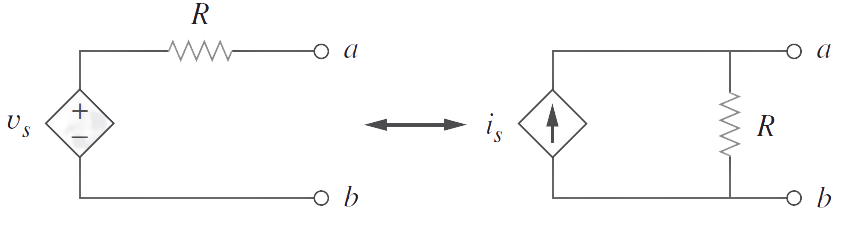
\includegraphics[width=1\textwidth]{transformacion} } \\
	 		
	 
	 \multicolumn{2}{l}{Transformación Estrella-Delta} 		\\
														& \multirow{4}{*}{\hspace{-.54cm} 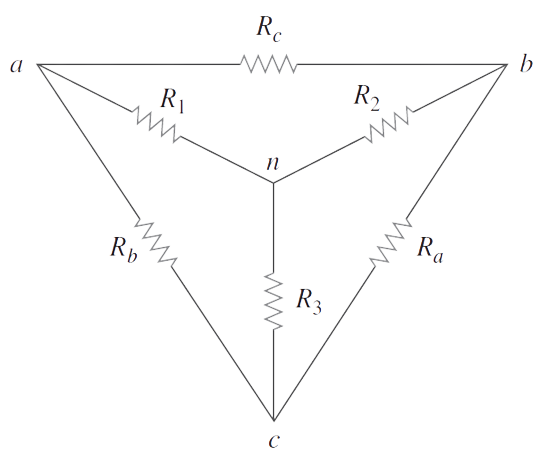
\includegraphics[width=.5\textwidth]{estrelladelta} }  \\
		  $R_{1}=\dfrac{R_{b}R_{c}}{R_{a}+R_{b}+R_{c}}$	&   \\ 
														& 	\\
		\hspace{-1cm}$R_{a}=\dfrac{R_{1}R_{2}+R_{2}R_{3}+R_{1}R_{3}}{R_{1}}$ \vspace{.5cm}	& \\
% HASTA ACÁ, PUEDEN SEGUIR CON NORMALIDAD DESPUÉS ;)
		
	\end{tabular} \\

		
			
		
%		\multicolumn{2}{c}{ } \\
%		Estrella-Delta & \\
%		\multicolumn{2}{c}{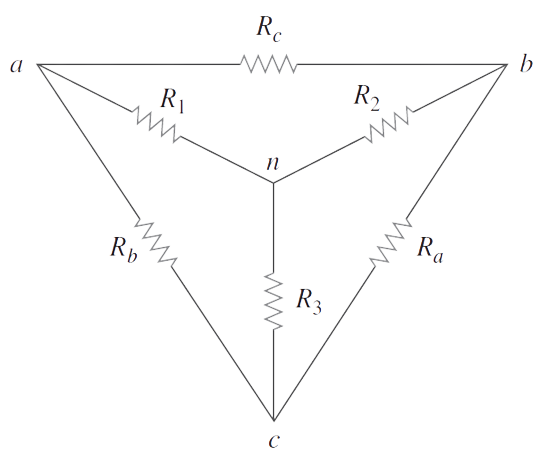
\includegraphics[width=.5\textwidth]{estrelladelta}} \\
%		\multicolumn{2}{c}{$R_{1}=\dfrac{R_{b}R_{c}}{R_{a}+R_{b}+R_{c}}$ \hspace{.2cm} $R_{a}=\dfrac{R_{1}R_{2}+R_{2}R_{3}+R_{1}R_{3}}{R_{1}}$}\\
%	
%\begin{tabular}{r l}
%
%\end{tabular}
		
	\textbf{\textsl{Supernodo: }} Fuente de tensión conectada entre dos nodos de no referencia. \\
	\textbf{\textsl{Superlazo: }} Dos lazos tienen una fuente de corriente en común.	
		
	
	
	
	\end{tcolorbox}

\newpage

\pagestyle{fancy}

\section*{Nomenclatura}
\begin{tabular}{r l}
	$f$ [1/s] & Frecuencia \\
	$\omega $ [$^{\circ}$/s] & Frecuencia angular \\
	$\fasor{V}$ [V]& Fasor de tensión \\
	$\fasor{I}$ [A]& Fasor de corriente \\
	$V_{m}$ [V] & Valor de tensión pico\\
	$I_{m}$ [A] & Valor de corriente pico \\
	$V_{rms}$ [V] & Valor de tensión eficaz\\
	$I_{rms}$ [A] & Valor de corriente eficaz \\
	$p(t)$ [W] & Potencia instantánea \\
	$S$ [VA] & Potencia aparente \\
	$\phi_{z}$ [ $^\circ$ ]& Ángulo de impedancia \\
	$\Re$ & Reluctancia\\
	
	
	
\end{tabular}


%%%%%%%%%%%%%%%%%%%%%%%%%% UNIDAD 1 ---------------------------------

\unidad{1}{Fasores}

	\begin{tcolorbox}[colback=white!97!brown, colframe=brown!15!gray]
		
	\textbf{Nota:} En general  para fasores se aplican los métodos ya conocidos, a diferencia de que ahora se trabajan con números complejos.\\

		
		Relación \textbf{reactancias-fasores }
\begin{center}		
		\begin{tabular}{r l}
			
			Reactancia &    Dominio de frecuencia\\ 
			$R=R$ & \fasor{V}$=R$\fasor{I}\\
			$ X_{L}= j \omega L $ & \fasor{V} $=X_{L}$ \fasor{I} \\
			$X_{C} = \dfrac{-j}{\omega C}$ & \fasor{V}$= - X_{C}$ \fasor{I} \\ \vspace{.1cm}
			Impedancia & $\fasor{Z}= R +j X$ \\
			Admitancia & $\fasor{Y} =\dfrac{1}{\fasor{Z}}=G + jB$ \\ 
			\multicolumn{2}{c}{$ G = \dfrac{R}{R^2+X^2} \hspace{.2cm} B=\dfrac{-X}{R^2+X^2} \hspace{.2cm} X=X_{L}-X_{C} $}
			\end{tabular}
\end{center}



	Leyes en \textbf{dominio frecuencial} (fasorial) \vspace{.1cm}

		\begin{tabular}{r l} \vspace{.1cm}
		Kirchhoff LTK & $\displaystyle\sum \fasor{V}=0$ \\ \vspace{.1cm}
		Kirchhoff LCK & $\displaystyle\sum \fasor{I}=0$ \\
		Ley de \textbf{Ohm} & $\fasor{V}=\fasor{I}\fasor{Z}$\\
		\vspace{.1cm}
		Circuitos en \textbf{serie} & 	$\fasor{Z}_{eq}=\displaystyle\sum \fasor{Z}$ \\ 
		Circuitos en \textbf{paralelo} & $\fasor{Y}_{eq}=\dfrac{1}{\fasor{Z}_{eq}}=\displaystyle\sum \dfrac{1}{\fasor{Z}}$ \\
		

		\multicolumn{2}{l}{\vspace{.2cm}Divisores de \textbf{tensión} y \textbf{corriente}} \\
		
	\hspace{-.4cm}	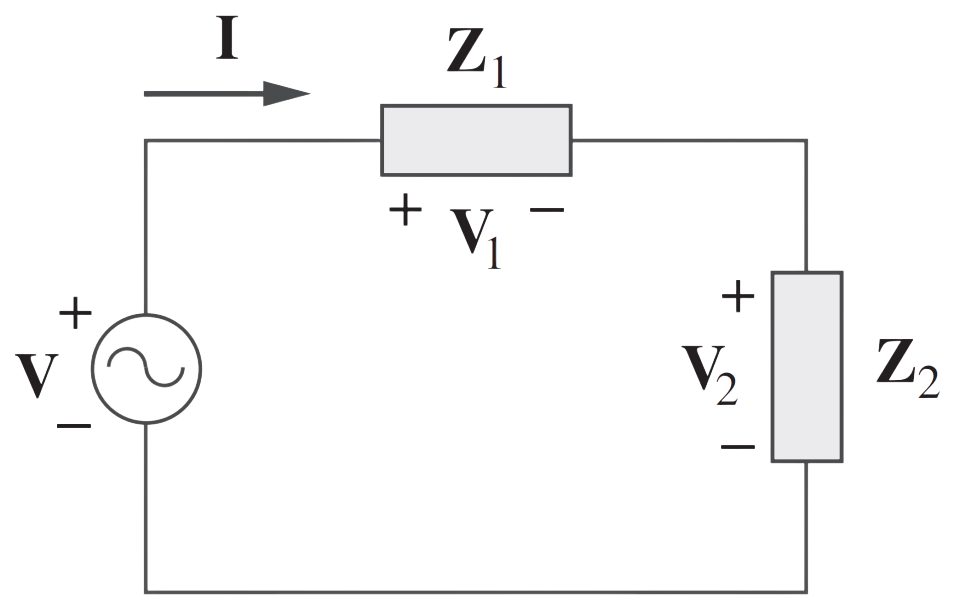
\includegraphics[width=.53\textwidth]{zserie}	& \hspace{-.35cm} 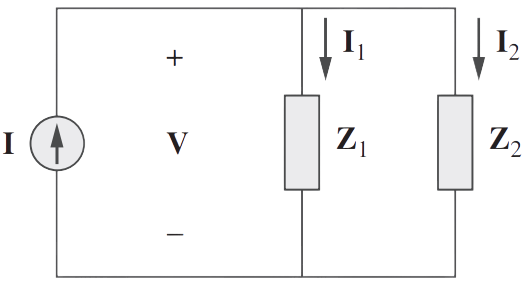
\includegraphics[width=.5\textwidth]{zparalelo} \\
	$\fasor{V}_{1} = \dfrac{\fasor{Z}_{1}}{\fasor{Z}_{1}+\fasor{Z}_{2}}\fasor{V}  $\hspace{.9cm} &  \vspace{.2cm}\hspace{.2cm} $ \fasor{I}_{1} = \dfrac{\fasor{Z}_{2}}{\fasor{Z}_{1}+\fasor{Z}_{2}}\fasor{I}  $ \\
	$ \fasor{V}=\displaystyle\sum \fasor{Z}_{i}\fasor{I}_{i} $ \hspace{.8cm} &  \hspace{.5cm} $ \fasor{I} =\displaystyle\sum \dfrac{\fasor{V}_{i}}{\fasor{Z}_{i}} $ \\
	
		
		\end{tabular}	

	\end{tcolorbox}


	\newpage

%%%%%%%%%%%%%%%%%%%%%%%%%% UNIDAD 2 ---------------------------------
	
\unidad{2}{Respuesta Natural}
	
	\begin{tcolorbox}[colback=white!97!brown, colframe=brown!15!gray]
	\begin{center}
		\textsc{Análisis con corriente directa}
	\end{center}
		Circuitos de\textbf{ primer orden}
		
		\begin{tabular}{r l}
			
			LTK en RL & $i_{n}(t)=A e^{\frac{-t}{\tau}}$ donde $\tau=\dfrac{L}{R}$ \\
			LCK en RC & $v_{n}(t)=A e^{\frac{-t}{\tau}}$ donde $\tau=RC$
			
		\end{tabular}\\
	
		Circuitos de\textbf{ segundo orden}
		
		\begin{tabular}{r l}\vspace{.2cm}	
		 	Raíces & $s_{1-2}=-\alpha\pm \sqrt{\alpha^{2}-\omega_{0}^{2}}$\\
	 		Frecuencia angular & $\omega = 2 \pi f = 2 \pi \dfrac{1}{\tau} $\vspace{.2cm}\\ 
	
			\multicolumn{2}{l}{Circuito RLC \textsl{en serie} (\textbf{LTK})} \\
			\multicolumn{2}{c}{$iR+L\dfrac{di}{dt}+\dfrac{1}{C}\displaystyle\int_{-\infty}^{t}idt=0 $} \vspace{.2cm} \\ 
			\multicolumn{2}{c}{$\dfrac{di}{dt}R+L\dfrac{d^2i}{dt^2}+\dfrac{i}{C}=0 $} \vspace{.2cm} \\ 
			\multicolumn{2}{c}{$\forall t=0$ $\rightarrow$ $i(0)R+L\dfrac{di(0)}{dt}+V_{0}=0 $} \vspace{.2cm}\\
			
			 \multicolumn{2}{c}{$\alpha=\dfrac{R}{2L}$ \hspace{.4cm} $\omega_{0}=\dfrac{1}{\sqrt{LC}}$ \hspace{.4cm}  $\omega_{d}=\sqrt{\omega^{2}-\alpha^{2}}$\vspace{.2cm}} \\
			 
			
			\multicolumn{2}{l}{Circuito RLC \textsl{en paralelo} (\textbf{LCK})} \\
			
			\multicolumn{2}{c}{$\dfrac{v}{R}+\dfrac{1}{L}\displaystyle\int_{-\infty}^{t}v dt+C\dfrac{dv}{dt}=0 $} \vspace{.2cm} \\ 
			
			\multicolumn{2}{c}{$\dfrac{1}{R}\dfrac{dv}{dt}+\dfrac{1}{L} v +C\dfrac{d^2 v}{dt^2}=0 $} \vspace{.2cm} \\ 
			
			
			\multicolumn{2}{c}{$\forall t=0$ $\rightarrow$ $\dfrac{v(0)}{R}+C\dfrac{dv(0)}{dt}+I_{0}=0 $} \vspace{.2cm}\\
			\vspace{-.5cm} & \\  %Esto agregué para separar un poco las líneas
			
			\multicolumn{2}{c}{$\alpha=\dfrac{1}{2RC}$ \hspace{.4cm}  $\omega_{0}=\dfrac{1}{\sqrt{LC}}$ \hspace{.4cm}  $\omega_{d}=\sqrt{\omega^{2}-\alpha^{2}}$\vspace{.2cm}} \\ 
			 
			\multicolumn{2}{l}{Funciones para la ED} \\ 
			
		sobre. $\alpha > \omega_{0}$ &$f(t)=A_{1}e^{s_{1}t}+A_{2} e^{s_{2}t}$ \vspace{.1cm}\\
			
		crit. $\alpha = \omega_{0}$&$f(t)=(A_{1}+A_{2}t)e^{-\alpha t}$ \vspace{.1cm}\\
			
		sub. $\alpha < \omega_{0}$ & $f(t)=Ae^{-\alpha t}\sin(\omega_{d}t+\theta)$ \vspace{.1cm}\\
			& $s_{1-2}=-\alpha + \omega_{d}j$\\
		\end{tabular}\\
	
	\textbf{Nota: } En las ecuaciones se puede utilizar $f(t)\equiv i(t)$ ó $v(t)$ sin importar si el circuito paralelo o en serie.
	\end{tcolorbox}
	

%%%%%%%%%%%%%%%%%%%%%%%%%% UNIDAD 3 -------------------------------	
	
\unidad{3}{Respuesta Forzada}
	
	\begin{tcolorbox}[colback=white!97!brown, colframe=brown!15!gray]
		La respuesta forzada o en \emph{estado estable} es producida por una 'fuerza' externa, no se extingue con el tiempo.
		
		\begin{tabular}{r l}
			En un capacitor & $v_{f}=v(\infty)$ \\
			En un inductor & $i_{f}=i(\infty)$ \\
		\end{tabular}
	\end{tcolorbox}

\newpage


\unidad{3}{Respuesta Forzada}

\begin{tcolorbox}[colback=white!97!brown, colframe=brown!15!gray]
	\begin{center}
		\textsc{Análisis con corriente alterna}
	\end{center}
	
	Circuitos de \textbf{primer orden}
	
	\begin{tabular}{r l}
		Dominio temporal & Dominio fasorial \\ \vspace{.1cm}
		$v(t) = V_{m} cos(\omega t + \phi_v )$ & $\fasor{V}=V_{rms} \phase{\phi_v}$ \\  \vspace{.1cm}
		$i(t) = I_{m} cos(\omega t + \phi_i)$ &  $ \fasor{I} = I_{rms}  \phase{\phi_i}$ \\ \vspace{.2cm}
		Circuito inductivo & $\fasor{I}= I_{rms} \phase{\phi_v -\theta}$ \\ \vspace{.2cm}
		Circuito capacitivo & $\fasor{I}=I_{rms} \phase{\phi_v + \theta}$ \\ 
		\multicolumn{2}{c}{$ V_{rms}=\dfrac{V_{m}}{\sqrt{2}} \hspace{.4cm} I_{rms}=\dfrac{I_{m}}{\sqrt{2}} $}
	\end{tabular}
	
	
\end{tcolorbox}

%%%%%%%%%%%%%%%%%%%%%%%%%% UNIDAD 4 ---------------------------------

\unidad{4}{Respuesta Completa}
	\begin{tcolorbox}[colback=white!97!brown, colframe=brown!15!gray]
	Circuitos de primer orden
	

		\begin{tabular}{r l}
		$i(t)=i_f+i_n$ &  $=i(\infty)+[i(\infty)-i(0)]e^{\frac{-t}{\tau}}$\\ \vspace{.2cm}
		$v(t)=v_{f}+v_{n}$ & $=v(\infty)+[v(\infty)-v(0)]e^{\frac{-t}{\tau}}$
		\end{tabular}

	
	Circuitos de segundo orden
	
	\begin{tabular}{r l}
		Serie & $i(t)=i_f+i_n=i(\infty)+i_{n}(t)$ \\
		Paralelo & $v(t)=v_f+v_n=v(\infty)+v_{n}(t)$
	\end{tabular}\\


	\textbf{Importante: }Las constantes se determinan con los valores iniciales y se utiliza la función de respuesta completa.
	\begin{center}
		$i(0) \hspace{.2cm} v(0)  \hspace{.2cm} \dfrac{di(0)}{dt} \hspace{.2cm}  \dfrac{dv(0)}{dt}$
	\end{center}
	
	\end{tcolorbox}
	
	
%%%%%%%%%%%%%%%%%%%%%%%%%% UNIDAD 5--------------------------------	
	
\unidad{5}{Potencia y Energía en Circuitos Monofásicos}
	\begin{tcolorbox}[colback=white!97!brown, colframe=brown!15!gray]
		
		\begin{tabular}{r l}
			
			Potencia instantánea & $p(t)=v(t)i(t)$ v\\
			Potencia promedio & $P=\displaystyle\int_{0}^{T} p(t) dt$ \\
			\textbf{Factor de potencia} & $fp=cos(\phi_{z}) \hspace{.3cm} $ \\
			& $\fasor{Z}=\dfrac{V_{m}}{I_{m}}\phase{\phi_{z}}$ \\
			Potencia aparente & $S=V_{rms}I_{rms}$ \\
%			Potencia compleja & $\fasor{S}=V_{rms}I_{rms} \phase{\theta_v -\theta_i}$ \\
			Potencia compleja & $\fasor{S}=\fasor{V} \times \fasor{I}$ \\
			Potencia real & $P=$Re$(\fasor{S})$ \\
			Potencia reactiva & $Q=$Im$(\fasor{S})$ \\
		\end{tabular}
		
	\end{tcolorbox}


\newpage

%END_FOLD

%	unidades 6 a 
%BEGIN_FOLD

%%%%%%%%%%%%%%%%%%%%%%%%%% UNIDAD 6 ---------------------------------

\unidad{6}{Redes eléctricas}
\begin{cajita}

Método de \textbf{mallas}

Se asigna un sentido a la corriente y se escriben las ecuaciones

\begin{center}
	
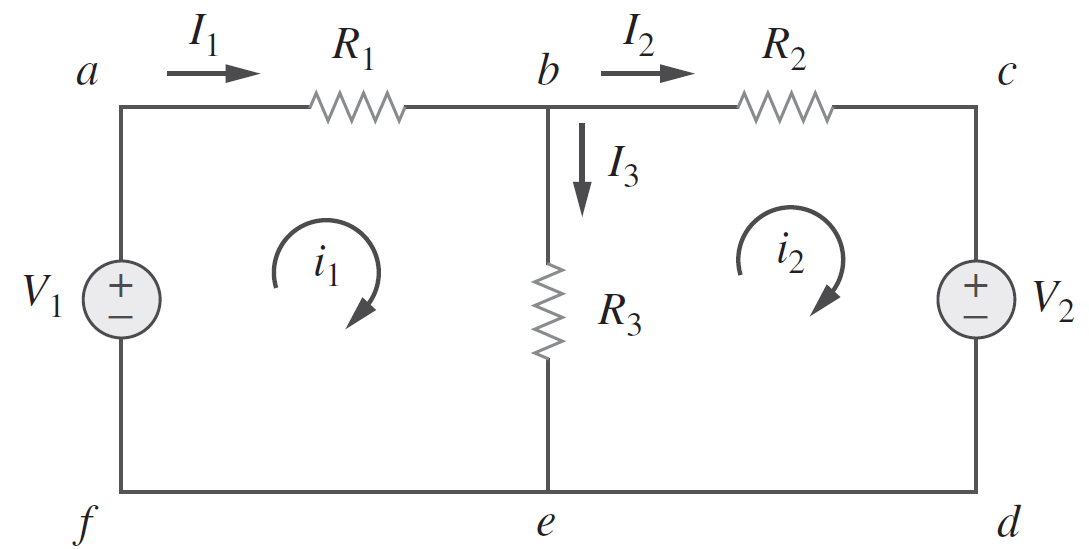
\includegraphics[width = 0.9\textwidth]{mallas}
\vspace{-.3cm}
\begin{equation}
	\begin{pmatrix}
		R_1 + R_3 & - R_3 \\
		- R_3 	& R_2 + R_3
	\end{pmatrix} \begin{pmatrix}
	i_1 \\
	i_2
\end{pmatrix} = \begin{pmatrix}
	V_1 \\
	- V_2
\end{pmatrix}
\end{equation}

\end{center}



Método de \textbf{nodos}

\vspace{0.1cm}
Teorema de \textbf{Thevenin}\\
\textit{``Cualquier red de corriente directa lineal bilateral de dos terminales puede ser reemplazada por un circuito equivalente que conste de una fuente
de voltaje y un resistor en serie''}
\vspace{0.1cm}


Teorema de \textbf{Norton}\\
\textit{ ``Cualquier red de cd lineal bilateral de dos terminales puede ser reemplazada	por un circuito equivalente que consista de una fuente de corriente y un
	resistor en paralelo''}
\vspace{0.1cm}
Teorema de \textbf{superposición}\\
\textit{``La corriente o el voltaje de un elemento en una red lineal bilateral es igual a la suma algebraica de las corrientes o voltajes producidos independientemente por cada fuente.''}\\
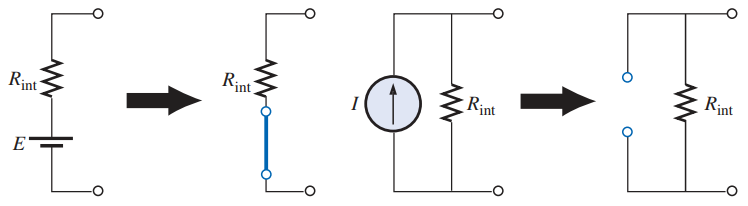
\includegraphics[width = 0.9\textwidth]{superposicion}
\vspace{-.3cm}
\vspace{0.1cm}
Teorema de \textbf{máxima transferencia de potencia}
	
	
\end{cajita}

\newpage
%%%%%%%%%%%%%%%%%%%%%%%%%% UNIDAD 7 ---------------------------------


\unidad{7}{Potencia polifásica}
\begin{cajita}
	
	Diferencia de potencial entregada por el generador
	\begin{center}
		
		\begin{tabular}{l l}
			\multicolumn{2}{c}{\textsl{Sistema \textbf{ABC}}} \\ \vspace{.2cm}
			$V_{AB} = V_{L} \phase{120^\circ}$ & $V_{AN} = V_F \phase{90^\circ} $ \\  \vspace{.2cm}
			
			$V_{BC}=V_L \phase{0}$ & $V_{BN} = V_F \phase{-30^\circ}$ \\ \vspace{.2cm}
			
			$V_{CA} = V_L \phase{-120^\circ}$ & $V_{CN} = V_F \phase{-150^\circ}$  \\
			
			%%%%%%%%%%%%%%%%%%%%
			\multicolumn{2}{c}{\vspace{.2cm} \textsl{Sistema \textbf{CBA}}} \\
			
			$ V_{AB} = V_L \phase{-120^\circ}$ & $V_{AN} = V_F \phase{-90^\circ} $\\ \vspace{.2cm}
			
			$V_{BC}=V_L \phase{0}$ & $V_{BN} = V_F \phase{30^\circ}$ \\ \vspace{.2cm}
			
			$V_{CA} = V_L \phase{120^\circ}$& $V_{CN} = V_F \phase{150^\circ} $\\
			
		\end{tabular}
	\end{center}
	
	\vspace{.3cm}
	
	Relación de impedancias. \textsc{cargas equilibradas}  \begin{center}
		\vspace{-.4cm}
		$Z_{\bigtriangleup} = 3 \cdot Z_\textup{Y}$
	\end{center}
	
	\vspace{.3cm}
	
	Relación conexión estrella-triángulo. \textsc{cargas equilibradas}
	\begin{center}
		\vspace{-.5cm}
		\begin{tabular}{l l || l l}
			\multicolumn{2}{c}{Conexión \textbf{estrella}} & \multicolumn{2}{c}{\vspace{.2cm}Conexión \textbf{triángulo}} \\ \vspace{.2cm}
			$V_L = \sqrt{3} V_F$ & $I_L = I_F$ & $V_L = V_F$ & $I_L = \sqrt{3} I_F$ \\ 
			\multicolumn{4}{c}{\vspace{.2cm} $P_T = 3 P_F = \sqrt{3} \cdot V_L \cdot I_L \cdot \cos \phi$}
		\end{tabular}
	\end{center}

	\vspace{.3cm}
	
	Equivalente monofásico. \textsc{cargas equilibradas} en estrella.
	
	%	Se considera la tensión de fase con ángulo cero y la impedancia en estrella. 
	
	\begin{center}
		$ I_L = \dfrac{V_F \phase 0^\circ}{Z_\textsc{Y}\phase {\phi}} = I_L \phase{-\phi}$
	\end{center}
	% Las corrientes tendrán módulo $I$, y estarán \textbf{desfasadas} respecto de \textbf{su tensión} un ángulo de valor $\phi$.
	
	\begin{center}
		\begin{tabular}{l l}
			$V_{fase} = V_F \phase {\theta_{F}} $ & $ I_{linea} = I_L \phase{\theta_{F} - \phi} $ \\
		\end{tabular}
	\end{center}
	
	\vspace{.3cm}
	
	Desplazamiento del punto neutro. \\
	\textsc{cargas desequilibradas.}
	\begin{center}
		$V_\textsc{on} = \dfrac{ V_\textsc{an}  Y_\textsc{a}  + V_\textsc{bn}  Y_\textsc{b} + V_\textsc{cn}  Y_\textsc{c} }{ Y_\textsc{a}  +Y_\textsc{b}   + Y_\textsc{c} }$
	\end{center}
	
\end{cajita}
	
	
%%%%%%%%%%%%%%%%%%%%%%%%%% UNIDAD 8 ---------------------------------

\newpage
\unidad{8}{Circuito magnético}
\begin{cajita}
	\begin{center}
		
		\begin{tabular}{r l}
			Fuerza Magnetomotriz & $F_m = N \cdot I$ \\
								& $F_m = H_i \cdot l_i $\\
			Flujo magnético & $\phi = B \cdot S$ \\
			Ley de Hopkinson & $F_m = \phi \cdot \Re$ \\			
			Densidad de flujo magnético & $B = \mu H$\\
						& $\mu = \mu_{0} \cdot \mu_{r}$\\
		\end{tabular}
		

	\end{center}	

	\begin{gather*}
		\Phi=\dfrac{N \cdot I}{\dfrac{l_{m}}{\mu_{0} \cdot \mu_{r} \cdot S}}=\dfrac{F_m}{\Re} \\	
		\intertext{En CA:}		
		\Phi (t) = \Phi_{max} \cos(\omega t - 90) 	\\
		\Phi_{max} = \dfrac{\sqrt{2} V_{ef}}{N \omega}	\\
		\intertext{De aca podemos obtener la tension eficaz.}
	\end{gather*}
	\textbf{Circuito equivalente de una bobina con nucleo de hierro}\\
	\hspace{.5cm}Nucleo sin perdidas\\
	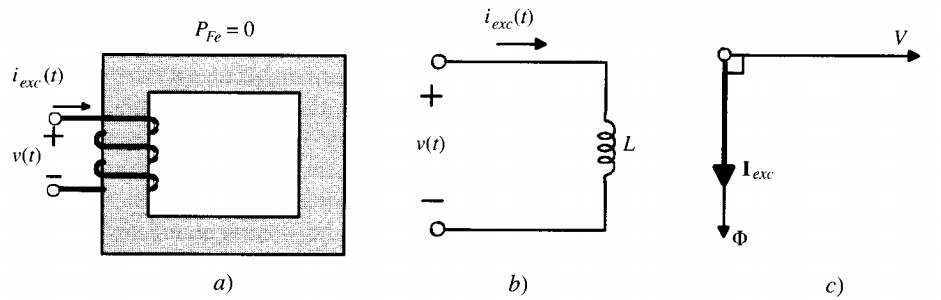
\includegraphics[width=.9\linewidth]{nucleoSP}
	\begin{gather*}
		\Phi = \dfrac{F_m}{\Re} = \dfrac{N \cdot I_{ex}}{\dfrac{l_{m}}{\mu \cdot S}} = \mu \dfrac{N I_{ex}}{l_{m}} S\\
		v = N \dfrac{d \Phi}{dt} = \dfrac{N^{2} S \mu}{l_{m}} \dfrac{dI_{ex}}{dt} = L \dfrac{dI_{ex}}{dt}
	\end{gather*}
	\hspace{.5cm}Nucleo con perdidas\\
	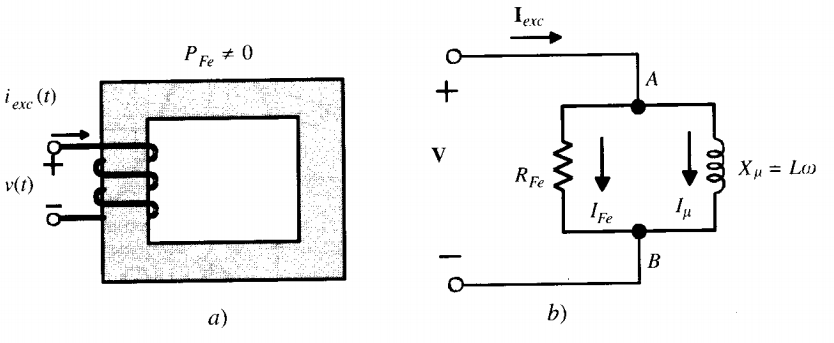
\includegraphics[width=.9\linewidth]{nucleoCP}
	\begin{center}
		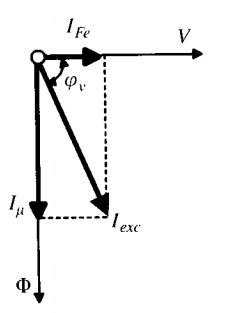
\includegraphics[width=.4\linewidth]{nucleoCP2}
	\end{center}

%A tener presente: $V=L.\dfrac{di}{dt}=N.\dfrac{d\phi}{dt}$\\
\begin{tabular}{r l}
	Mutua inductancia& $M=k\sqrt{L_1 L_2}$\\
					&$k=\frac{\phi_{12}}{\phi_{1}}=\frac{\phi_{21}}{\phi_{2}} $\\
					&$L_1=\frac{\phi_{1}}{i_{1}} $\\
					&$L_2=\frac{\phi_{2}}{i_{2}} $\\
\end{tabular}

Regla de los puntos para M:\\
\textit{``Si las dos corrientes entran o salen de las bobinas por los terminales con punto, los signos de los términos en M son los mismos que los de los términos en L. Si una entra por un terminal con punto y la otra sale por el otro terminal con punto, los signos de los términos en M son opuestos a los de L''}.\\
Análogamente: \textit{``Si la corriente en la bobina inductora entra por el extremo punteado la tensión inducida será positiva en el extremo punteado de la bobina inducida''}
	
\end{cajita}
%END_FOLD
\newpage
\unidad{nro}{Componentes simétricos}
\begin{cajita}
	\begin{center}
		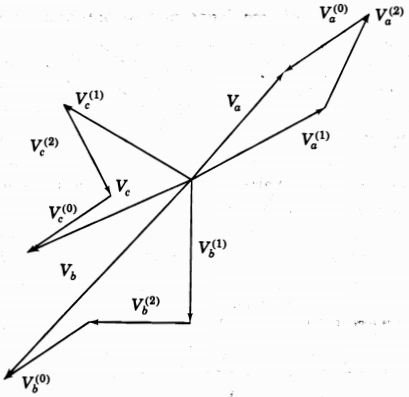
\includegraphics[width=4cm]{simetricos1}

	\resizebox{ 7 cm}{!} { %ACA REESCALA LA TABLA 
	\begin{tabular}{l l}
		\begin{tabular}{l}
			$V_{a}=V_{a}^{0}+V_{a}^{1}+V_{a}^{2}$\\
			$V_{b}=V_{a}^{0}+\alpha^{2}V_{a}^{1}+\alpha V_{a}^{2}$\\
			$V_{c}=V_{a}^{0}+\alpha V_{a}^{1}+\alpha^{2}V_{a}^{2}$
		\end{tabular} & 
		\begin{tabular}{l}
			$I_{a}=I_{a}^{0}+I_{a}^{1}+I_{a}^{2}$\\
			$I_{b}=I_{a}^{0}+\alpha^{2}I_{a}^{1}+\alpha I_{a}^{2}$\\
			$I_{c}=I_{a}^{0}+\alpha I_{a}^{1}+\alpha^{2}I_{a}^{2}$
		\end{tabular}\\
	\end{tabular}%
	}
\end{center}

Expreso en forma matricial:

\begin{center}
	$\left[ 
	\begin{array}{c}
		X_{a}\\		X_{b}\\		X_{c}
	\end{array}
	\right] 
	=
	\left[ 
	\begin{array}{c c c}
		1&1&1\\
		1&\alpha^{2}&\alpha\\
		1&\alpha&\alpha^{2}
	\end{array}
	\right] 
		\left[ 
	\begin{array}{c}
		X_{a}^{(0)}\\		X_{a}^{(1)}\\		X_{a}^{(2)}
	\end{array}
	\right]$\\
	
		$\left[ 
	\begin{array}{c}
			X_{a}^{(0)}\\ X_{a}^{(1)}\\	X_{a}^{(2)}
	\end{array}
	\right] 
	= \frac{1}{3}
	\left[ 
	\begin{array}{c c c}
		1&1&1\\
		1&\alpha&\alpha^{2}\\
		1&\alpha^{2}&\alpha
	\end{array}
	\right] 
	\left[ 
	\begin{array}{c}
		X_{a}\\		X_{b}\\		X_{c}
	\end{array}
	\right]$
\end{center}
	\textbf{Redes de secuencia}\\
\begin{tabular}{c c}
	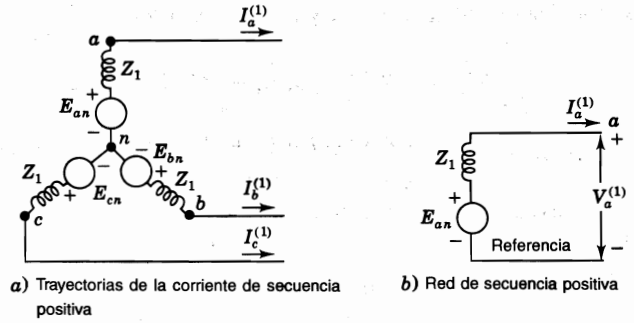
\includegraphics[width=4cm]{rspositiva}& $  V_{a}^{(1)}= E_{an} -I_{a}^{1}.Z_{1}$\\
	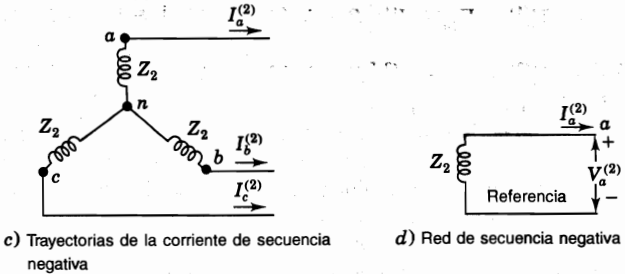
\includegraphics[width=4cm]{rsnegativa}& $  V_{a}^{(2)}= 0 -I_{a}^{2}.Z_{2}$\\
	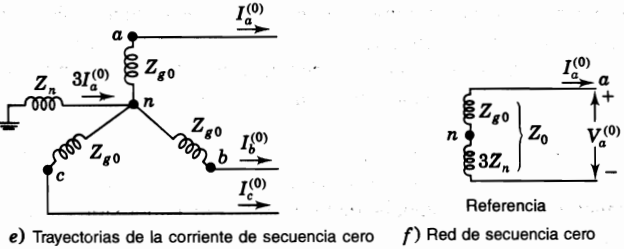
\includegraphics[width=4cm]{rscero}& $  V_{a}^{(0)}= 0 -I_{a}^{0}.Z_{0}$
\end{tabular}

%			V_{a}^{(0)}\\ V_{a}^{(1)}\\	V_{a}^{(2)}
%	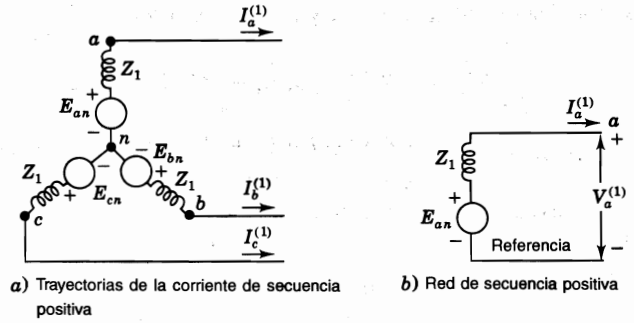
\includegraphics[width=4cm]{rspositiva}\\
%	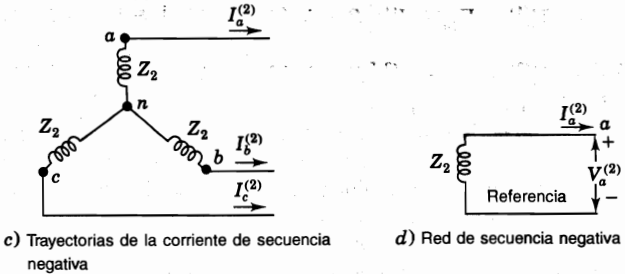
\includegraphics[width=4cm]{rsnegativa}\\
%	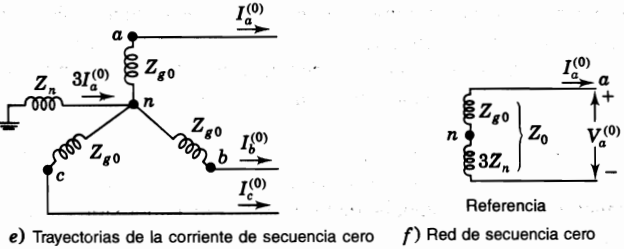
\includegraphics[width=4cm]{rscero}\\
\textbf{Fallo de 1 línea a tierra}\\
Condiciones : $ I_{b}=I_{c}=0~,~V_{a}=0 $
\begin{center}
	\vspace{-0.2cm}
	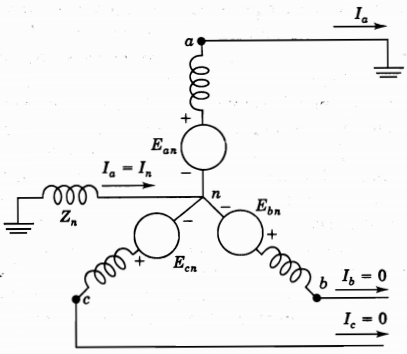
\includegraphics[width=3cm]{f1lg}\\
	\boxed{I_{a}^{0}=I_{a}^{1}=I_{a}^{2}=\dfrac{Ea}{Z_{1}+Z_{2}+Z_{0}}}
\end{center}
%%\[
%Ese corchete es lo mismo que usar $ $.. dato... por si te interesa
%%\]
\end{cajita}
\newpage
\begin{cajita}

	\textbf{Fallo de linea a linea punto}\\
	Condiciones : $I_{a}=0~,~ I_{b}=-I_{c}~,~V_{b}=V_{c}=0? $
	\begin{center}
		\vspace{-0.2cm}
		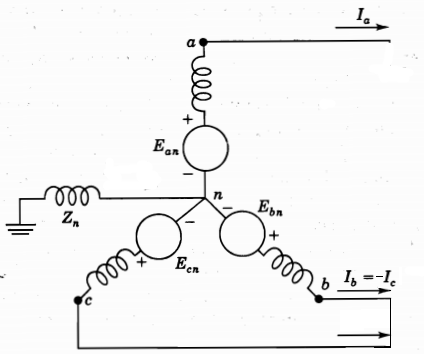
\includegraphics[width=5cm]{f1ll}\\
		\boxed{I_{a}^{1}=-I_{a}^{2}=\dfrac{Ea}{Z_{1}+Z_{2}}}
	\end{center}
	\textbf{Fallo de linea a linea punto}\\
	Condiciones : $I_{a}=0~,~ I_{b}=-I_{c}~,~V_{kb}-V_{kc}=I_{fb}Z_{f} $
	\begin{center}
		\vspace{-0.2cm}
		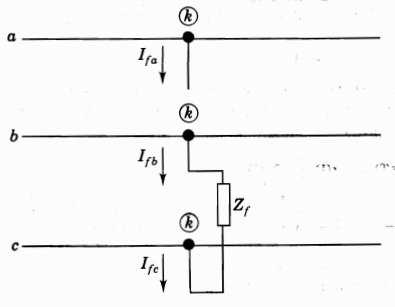
\includegraphics[width=3cm]{f2ll}\\
		\boxed{I_{a}^{1}=-I_{a}^{2}=\dfrac{Ea}{Z_{1}+Z_{2}+Z_{f}}}
	\end{center}

	\textbf{Fallo de doble linea a tierra punto}\\
	Condiciones : $I_{a}=0~,~ V_{b}=V_{c}=0~ $
	\begin{center}
		\vspace{-0.2cm}
		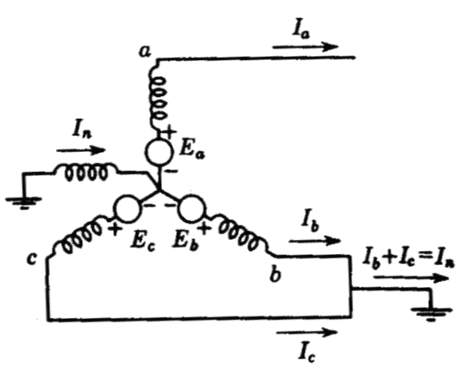
\includegraphics[width=3cm]{f2lg}\\
		\boxed{I_{a}^{1}=\dfrac{Ea}{Z_{1}+Z_{2}||Z_{0}}}
	\end{center}
\end{cajita}
\end{document}